
%--------------------------------- page style --------------------------------
\documentclass[12pt]{article}
\usepackage[dvips]{graphics}
\usepackage[english]{babel}
\usepackage{doublespace}
\usepackage{epsf}
\usepackage{fancybox}
\usepackage{fancyheadings}
\usepackage{float}
\usepackage{graphicx}
\usepackage{here}
\usepackage{isolatin1}
\usepackage{palatino}
\usepackage{picinpar}
\usepackage{psfig}
\usepackage{rotate}
\usepackage{subfigure}
\usepackage{sverb}
\usepackage{t1enc}
\usepackage{wrapfig}


\setlength{\topmargin}{0cm}
\setlength{\headheight}{1cm}
\setlength{\textheight}{23cm}
\setlength{\textwidth}{16cm}
\setlength{\oddsidemargin}{0cm}
\setlength{\evensidemargin}{0cm}
\setlength{\columnsep}{0.125in}
\setlength{\columnseprule}{0.5pt}
\setlength{\footskip}{1cm}
\setstretch{1}

%--------------------------------- styles--------------------------------
%
% Setting the width of the verbatim parts according to 80 tt chars
% Since it is tt, any char is fine
%
\newlength{\verbatimbox}
\settowidth{\verbatimbox}{\scriptsize\tt
xxxxxxxxxxxxxxxxxxxxxxxxxxxxxxxxxxxxxxxxxxxxxxxxxxxxxxxxxxxxxxxxxxxxxxxxxxxxxxxx
}

\newenvironment{sourcelisting}
  {\VerbatimEnvironment\par\noindent\scriptsize
   \begin{Sbox}\begin{minipage}{\verbatimbox}\begin{Verbatim}}%
  {\end{Verbatim}\end{minipage}\end{Sbox}

\setlength{\fboxsep}{3mm}\center\shadowbox{\TheSbox}\normalsize\par\noindent}

\newenvironment{commandline}
  {\VerbatimEnvironment\par\vspace*{2mm}\noindent\footnotesize
   \begin{Sbox}\begin{minipage}{.979\textwidth}\begin{Verbatim}}%
  {\end{Verbatim}\end{minipage}\end{Sbox}\setlength{\shadowsize}{2pt}%
  \shadowbox{\TheSbox}\normalsize\par\noindent}

\rfoot{\thepage}
\lfoot{ALLIANCE TUTORIAL}
\cfoot{}
\setlength{\footrulewidth}{0.6pt}

%--------------------------------- page style --------------------------------
\pagestyle{fancy}
\rhead{VHDL Modeling and simulation}
\lhead{PART 1}
\rfoot{\thepage}
\lfoot{ALLIANCE TUTORIAL}
\cfoot{}
\setlength{\footrulewidth}{0.6pt}

%---------------------------------- document ---------------------------------

\begin{document}

\title{
                    {\Huge ALLIANCE TUTORIAL\\}
	 {\large
               Pierre \& Marie Curie University \\
                    year 2001 - 2004\\
    }
    \vspace{1cm}
    {\huge
                      PART 1\\
                Simulation
    }
}
\date{}
      
\author{Frederic AK \hspace{2cm}  Kai-shing LAM\\
Modified by LJ
}

\maketitle

\begin{figure}[H]\centering
  \includegraphics[height=7cm]{cpt3.epsi}
\end{figure}

\begin{figure}
\end{figure}

\thispagestyle{empty}
\def\myfbox#1{\vspace*{3mm}\fbox{#1}\vspace{3mm}}

        \vspace{3cm}


\newpage
\large{ The purpose of this tutorial is to provide a quick turn of some { \bf
ALLIANCE } tools, developed at the LIP6 laboratory of Pierre and Marie Curie
University.

The tutorial is composed of 3 main parts independent from each other:

\begin{itemize}\itemsep=-.8ex
\item {VHDL modeling and simulation}
\item {Logical synthesis}
\item {Place and route}
\end{itemize}

Before going further you must ensure that all the environment variables are
properly set (source alcenv.sh or alcenv.csh file)
and that the Alliance tools are available when invoking them at the shell
prompt.

All the tools used in this tutorial are documented at least with a
manual page.

\newpage
{\bf Contents}\\
\\
{1} {\bf Behavioral VHDL}

{1.1} Introduction

{1.2} Behavioral Description

{1.3} Stimuli format

{1.4} Simulation

{1.5} Simulation with Delay\\
\\
{2} {\bf Structural VHDL}

{2.1} Introduction

{2.2} Stimuli Generation

{2.3} Structural View

{2.4} Structural view and validation of each block

{2.5} Simulation and validation of the addaccu on 2 hierarchical levels

\newpage
        {\huge
        PART 1 :\\ }
        \vspace{1cm}
        {\huge
        VHDL modeling and simulation
        }

All the files used in this part are located in the \\ 
\texttt{/tutorial/simulation/src} directory.\\
This directory contains two subdirectories and one Makefile : 
\begin{itemize}
\item The Makefile allows you to validate automatically the entire simulation part
\item {\bf addaccu\_beh} = the behavioral description (Register Transfert Level)

\begin{itemize}
\item Makefile to validate automatically the entire behavioral description
\item addaccu.vbe is the behavioral description of addaccu
\item patterns.pat is the simulation patterns for addaccu
\item addaccu\_dly.vbe is the behavioral description of addaccu with delay
\item patterns\_dly.pat is the simulation patterns for addaccu with delay
\item addaccu4.vhdl is the behavioral description of addaccu using standard VHDL subset
\end{itemize}

\item {\bf addaccu\_struct} = the structural view 

\begin{itemize}
\item Makefile to validate automatically the entire structural view
\item pat\_new.c is the vectors generation file
\item addaccu.vbe is the behavioral description of addaccu
\item mux.vbe is the behavioral description of multiplexer
\item accu.vbe is the behavioral description of accumulator
\item alu.vbe is the behavioral description of adder
\item addaccu.vst is the structural view of addaccu
\item mux.vst is the structural view of multiplexer
\item accu.vst is the structural view of accumulator
\item alu.vst is the structural view of adder
\end{itemize}

\end{itemize}

The {\bf ALLIANCE} tools used are :
\begin{itemize}\itemsep=-.8ex
\item {\bf vasy} : {\bf VHDL} analyzer and convertor.
\item {\bf asimut} : {\bf VHDL} Compiler and Simulator.
\item{\bf genpat} :    Procedural generator of stimuli.
\end{itemize}

You can obtain the detailed informations on an any
{\bf ALLIANCE} tool by typing the command :

\begin{commandline}
 > man <tool name>
\end{commandline}

To validate the behavioral and the structural description you can :
\begin{itemize}
\item  run the {\bf UNIX} commands in the order indicated by this tutorial.
\item  validate automatically the entire behavioral (or structural) description using the command : 
\end{itemize}

\begin{commandline}
> make
\end{commandline}
If you want to start again this validation from the beginning,
you just have to type :
\begin{sourcelisting}
 > make clean
 > make
\end{sourcelisting}

\newpage
\section{Behavioral VHDL}

\subsection{Introduction}

The goal of this part is to write then to simulate the behavior
of a very small circuit :
An accumulating adder which we will call addaccu.

The description of the behavior of addaccu will be made
in {\bf Behavioral VHDL (DATAFLOW)}.

\subsection{Behavioral Description}

The behavioral description of a circuit consists on a continuation
of logical equation calculating the outputs according to the
inputs with the use of possible internal signals ; in our case, a
signal which connects the output of the accumulator to the entry
of the multiplexer (reg\_out), another which connects the output
of the multiplexer to the entry of the adder (mux\_out) and
finally a signal for carry (carry).

At first, you must write the file of behavioral description of addaccu.
This description must be of type : without delay (without After clause).

This file will have the extension ".vbe" which is the usual extension
to indicate a {\bf VHDL} behavioral file (Vhdl BEhaviour description).
This description will have three distinct parts:

\begin{itemize}\itemsep=-.8ex
\item {\bf Block 1} : The 4 bits adder.
\item {\bf Block 2} : The 4 bits multiplexer.
\item {\bf Block 3} : The 4 bits accumulator.
\end{itemize}

The circuit has the following interface:

\begin{itemize}\itemsep=-.8ex
\item  a 4 bits input bus a.
\item  a 4 bits input bus b.
\item  a 4 bits output bus S.
\item  a clock input signal ck.
\item  a control input signal sel.
\item  two alimentation inputs signals VDD and VSS.
\end{itemize}


\begin{figure}[H]
  \center
  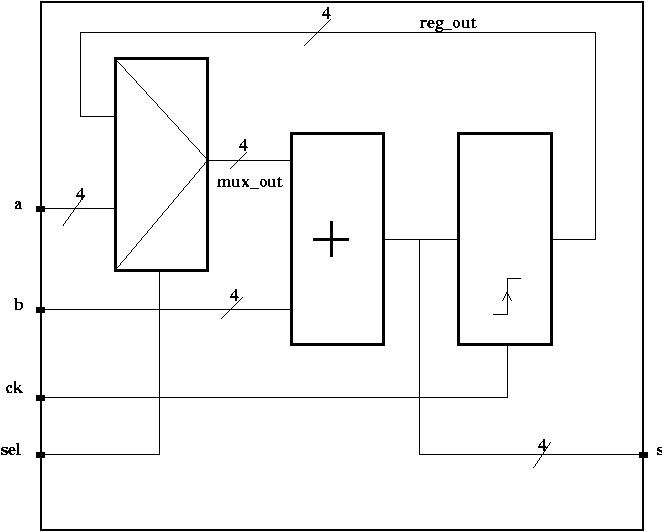
\includegraphics[width=.5\textwidth]{addac.eps}
  \caption{\bf accumulating adder }
\end{figure}

\begin{enumerate}
\item {\bf mux } is a 4 bits multiplexer 1 among 2\\
    {\bf mux} truth table : \\
    sel = 0 => mux\_out = a \\
    sel = 1 => mux\_out = reg\_out \\
\item {\bf alu} is a 4 bits adder \\
    s = b + mux\_out \\
\item {\bf accu} is a register (flip-flop) \\
    ck = 0 =$>$ reg\_out = reg\_out \\
    ck = 1 =$>$ reg\_out = reg\_out \\
    ck : 0-$>$1 =$>$ reg\_out = s \\
\end{enumerate}

Then you must validate your description while compiling with {\bf ASIMUT}.

\begin{commandline}
 > asimut -b -c <file name>
\end{commandline}

\begin{itemize}\itemsep=-.8ex
\item {\bf file name} is the file name of your behavioral description without
    extension ({\bf addaccu}).
\item {\bf -b} option to indicate that the description is purely behavioral.
\item{\bf -c} option to compile without simulating.
\end{itemize}

If you do not wish to use the environment variables positioned by
default, other environment variables can be used by {\bf ASIMUT}.

\begin{sourcelisting}
 > MBK_WORK_LIB = .
 > MBK_CATA_LIB = .
 > MBK_CATAL_NAME = CATAL
 > MBK_IN_LO = VST
\end{sourcelisting}

under Bash :
\begin{sourcelisting}
 > export var = value
\end{sourcelisting}

under standard Bourne Shell :
\begin{sourcelisting}
 > var = value
 > export var
\end{sourcelisting}

under C Shell :
\begin{sourcelisting}
 > setenv var value
\end{sourcelisting}

The meaning of these variables is to be discovered in the {\bf
man} of {\bf ASIMUT} tool.

\subsection{Description with Standard VHDL subset}

Alliance tools use a very particular and restricted {\bf VHDL} subset (vbe and
vst file format).

If you want to describe the behavior of your circuit (at Register Transfert Level)
with a more common {\bf VHDL} subset  you can use {\bf VASY\}
to automatically convert your {\bf VHDL} descriptions in 
Alliance subset.

The file addaccu4.vhdl is a description of the addaccu circuit,
using classical {\bf VHDL} subset (with process statements,
IEEE 1164 VHDL types, aritmetic operators etc ...) 

You can convert this description to the {\bf .vbe} file format using
 {\bf VASY}~:
\begin{commandline}
 > vasy -Vao addaccu4.vhdl
\end{commandline}

You can then compile and simulate the generated file addaccu4.vbe
using {\bf asimut} exactly as it has been done with the addaccu.vbe file.

\subsection{Stimuli of test}

Once the behavioral description compiled successfully (without any
error), to validate your description you must write a file of
nonexhaustive but intelligent vectors of test.

Therefore you must write a file {\bf patterns.pat} which contains a
dozen vectors of test. These vectors of test make it possible to
check that the adder makes the additions well with or without carry propagation ,
that the multiplexer gives the good operand to the input of the adder
following the value of {\bf sel} signal and finally, that the accumulator
correctly memorizes the output value of the adder.

In order not to have signals overlapping temporally (phenomenon of
" glitch "), you will use a clock with very high period (tck =
100ns) compared to the propagation times. The clock must respect the
following rate: 1 low state of 50 ns, then 1 high state of 50 ns,
etc...

If the {\bf PAT} syntax does not appear to you obvious, have a look to the
man giving the patterns files format : PAT format.

\begin{commandline}
 > man 5 pat
\end{commandline}


The {\bf 5} refers here to the class of handbooks for files formats.

\begin{itemize}\itemsep=-.8ex
\item {\bf man 1 }   : User Commands.
\item {\bf man 2,3 } : Libraries.
\item {\bf man 5 }   : Files format.
\item {\bf man 7 }   : Environment variables.
\end{itemize}


\subsection{Simulation}

Now you only have to simulate your addaccu with your vectors of
tests, without any delay in order to check very quickly that the
results on the outputs are well those which you wait.

\begin{commandline}
 > asimut -b addaccu patterns result_vbe
\end{commandline}

\begin{itemize}\itemsep=-.8ex
\item {\bf addaccu} : file name of the behavioral description 
      ({\bf addaccu.vbe}).
\item {\bf pattern} : file name of the vectors ({\bf pattern.pat}).
\item {\bf result\_vbe} : file name of the patterns result
      ({\bf result\_vbe.pat}).
\item {\bf -b} : option to indicate a purely behavioral description.
\end{itemize}

The file of resulting vectors must be seriously analyzed to check
the results of simulation. It is possible to use the graphical
pattern viewer {\bf xpat} to analyze the results of
the simulation.

\subsection{Delays}

The behavioral description written previously includes only
zero-delay concurrent assignements. It is however possible to
specify propagation times by using AFTER clauses, because the
operations in a real circuit are not done instantaneously. For
more details, do refer to the man for VBE files format.

You must modify your behavioral description to add delays :

\begin{itemize}\itemsep=-.8ex
\item For the adder : {\bf 4 ns}.
\item For the multiplexer : {\bf 2 ns}.
\item For the accumulator : {\bf 3 ns}.
\end{itemize}

The installation of the delay for the accumulator requires an
intermediate signal {\bf reg} because you cannot put delay on a
signal of {\bf register} type. In the test vectors file, it is
necessary to put the option {\bf spy} on the signals with delays
so that we can see these delays. In the contrary case,
these signals are sampled only at the times of the clock-edge.

Then you must validate this modified behavioral description while simulating
with { \bf asimut }.

\begin{commandline}
 > asimut -b addaccu_dly patterns_dly result_dly
\end{commandline}


The results obtained (result\_dly.pat) must be different from
those obtained without AFTER clauses (result\_vbe.pat). To
understand why, it is necessary to deeply analyze the temporal
behavior of your circuit. The step of 50 ns used for the test 
vectors does not really make possible to observe the true
temporal behavior of your circuit.  You can spy on all the
transitions from an internal signal or an output by specifying
this characteristic while declaring in the file of
test vectors (option { \bf spy }, for more details, consult the
man for patterns files format).


\newpage
\section{Structural VHDL}

\subsection{Introduction}


The goal of this part is to write then to simulate in a
hierarchical way the structural view of the circuit presented in
first part of this Tutorial. The circuit will be describe in two
levels of hierarchy :

\begin{itemize}\itemsep=-.8ex
\item The first level will write the circuit like the instanciation of three blocks.
\item The second level will write each of the three blocks in term
of elementary gates of the standard library.
\end{itemize}

Structural description of addaccu will be made in {\bf STRUCTURAL
VHDL }. 

This part contains five distinct steps:
\begin{itemize}\itemsep=-.8ex
\item {\bf step 1} : Generation of the complete set of vectors and validation of the addaccu.
\item {\bf step 2} : {\bf VHDL} structural description of the addaccu.
\item {\bf step 3} : Simulation and validation of the structural addaccu
                        on a hierarchical level.
\item {\bf step 4} : structural description and validation of each block.
\item {\bf step 5} : Simulation and validation of the structural addaccu
                        on 2 hierarchical levels.
\end{itemize}


\subsection{Stimuli Generation}

Normally, the behavioral description has been successfully compiled,
and validated with some hand made vectors.
Now you must create a file of test
vectors more consequent (a hundred clock-edges).

However, the writing of the stimuli file directly is a tiresome work.
The tool {\bf genpat} enables you to undertake this work in a
procedural way. The language {\bf genpat} is a subset of " C " functions.
For more informations on genpat and the functions of the
associated library do not hesitate to use the command:

\begin{commandline}
 > man genpat
\end{commandline}

Moreover, each basic function from {\bf genpat} has its man, the
functions are in capital letters, as by example:

\begin{commandline}
 > man AFFECT
\end{commandline}

Here are some suggestions for your file of vectors generation :

\begin{itemize}\itemsep=-.8ex
\item Write a function independent of the management of
      the clock. This clock will be synchronized on 2 times:
      a low state of 50 ns followed by a high state of 50 ns.
\item All the inputs of the circuit must be positioned in the first vector.
\item Initialize the accumulating register with the function {\bf INIT}.
\end{itemize}

Once your file {\bf pat\_new.c} is written you must compile it.
The following commands make it possible to compile the file of
procedural description and to generate the file of vectors
pat\_new.pat.

\begin{commandline}
 > genpat pat_new
\end{commandline}

If no error has occurred, the file {\bf pat\_new.pat} is now created.
You only have to simulate your behavioral addaccu
with this new set of vectors

\begin{commandline}
 > asimut -b -zerodelay addaccu pat_new res_new
\end{commandline}

The -zerodelay option states here that you wish a purely logical
simulation (without considering the propagation times). You obtain
then a file of vectors (res\_new.pat) result.

This file will be useful to you for the validation of the next
stages

\subsection{Structural View}

The objective here is to realize a hierarchy on one level by
making so that the structural view of the accumulating adder
addaccu.vst instancies the behavioral description of the 3 basic
components, the adder alu.vbe, the multiplexer mux.vbe and the
accumulator accu.vbe. \\
Initially you must write the structural
description file of addaccu. This file will have the extension "
vst " which is the usual extension to indicate a { \bf VHDL }
structural file (Vhdl Structural view). This view will contain the
instanciation of three independent blocks:

\begin{description}\itemsep=-.8ex
\item[Block 1] : The 4 bits adder.
\item[Block 2] : The 4 bits Multiplexer.
\item[Block 3] : The 4 bits accumulator.
\end{description}

You must create a {\bf CATAL} file containing the identifier of
each block followed by the attribute 'C' indicating that it is a
basic element of the hierarchy. This shows you the importance of
the {\bf CATAL} file which forces the simulator {\bf asimut} to
use the behavioral sight of the components which are listed. You
have to set the environment variable MBK\_IN\_LO:

\begin{sourcelisting}
 > MBK_IN_LO = vst
 > export MBK_IN_LO
\end{sourcelisting}

The meaning of all the usable variables is to be discovered in the
man of { \bf asimut } tool.

Lastly, validate your structural description while compiling with \\
{ \bf asimut }.

\begin{commandline}
 > asimut -c addaccu
\end{commandline}

Then simulate your circuit with the vectors file obtained
previously (the res\_new.pat file obtained by simulation
zero-delay of the behavioral description).

\begin{commandline}
 > asimut -zerodelay -nores addaccu res_new
\end{commandline}

The -nores option states here that you do not wait a result file.
When you do not have any more error of simulation you
will have to create the structural view of each of the 3 blocks.

\subsection{Structural view and validation of each block}

Now you have to pass to a hierarchy on 2 levels. So it is
necessary to write a structural view .vst for each basic component
of the accumulating adder and to test one by one replacing the
behavioral description of the basic components of the accumulating
adder by their structural views by modifying the {\bf CATAL} file 
(by removing the component name ).

Each block (alu, accu, mux) must now be described like an
interconnection of elementary gates. The gates which are to instanciate will
be chosen among those available in the library of standard cells {
\bf SXLIB }. For the functionality of the various cells and their
interface, the sxlib man is available. The behavioral
description of each cell is present in \\
{\bf /alliance/cells/sxlib }.

You must set the environment variable { \bf MBK\_CATA\_LIB }
to be able to reach these cells.

\begin{commandline}
 > MBK_CATA_LIB=/alliance/cells/sxlib
 > export MBK_CATA_LIB
\end{commandline}

For each block adopt following methodology to replace the
behavioral description of the block by its structural view:

\begin{itemize}\itemsep=-.8ex
\item Write the structural view of the block { \bf (vst) }.
\item
Compile this block (asimut -c $<$block\_name$>$) to validate its
syntax
\item Remove its identifier from the { \bf CATAL } file.
\item Simulate circuit addaccu again:  \par
\end{itemize}

\begin{commandline}
 > asimut -zerodelay -nores addaccu res_new
\end{commandline}

\subsection{Simulation and validation of the addaccu on 2 hierarchical levels}

Now you only have to simulate your addaccu described in a
hierarchical way (in which the basic elements are the library cells).

\begin{itemize}\itemsep=-.8ex
\item Erase the CATAL file, which is not necessary any more, the library of cells standards having its own catalogue.
\item Simulate again the addaccu circuit
\end{itemize}

\begin{commandline}
 > asimut addaccu pat_new res_dly
\end{commandline}

      Thus you will have replaced the behavioral description of the three blocks by their structural view.
\begin{itemize}\itemsep=-.8ex
\item You can again simulate the addaccu circuit in order to observe its temporal behavior
      precisely (each cell of the standard library has a given propagation time).
      You will use the { \bf spy } option for the internal signals and the outputs.
      
\end{itemize}

\begin{commandline}
 > asimut addaccu pat_new res_dly
\end{commandline}

\end{document}
